\documentclass{beamer}
\usetheme{Goettingen}
\usecolortheme{orchid}
\usefonttheme{structuresmallcapsserif}
\usepackage[utf8]{inputenc}
\usepackage{float}
\usepackage{fancybox} 
\usepackage{booktabs}
\setbeamertemplate{blocks}[rounded][shadow=true]
\usepackage{cancel}

\usepackage[USenglish]{babel}  
\usepackage{times}  
\usepackage{tikz}  
\usepackage{parskip}

\graphicspath{'X:/Users/Josh/Dropbox/poker/DC/3BP/Higher Level/Why we 3-bet/Isolate.png'}
%Information to be included in the title page:
\title{Why do we 3-bet?}
\subtitle{Part of a Comprehensive Guide to All Things Related to 3-Bets}
\author{Josh Plotkin}
\institute{DeucesCracked.com}
\date{}

\AtBeginSection[]
{
  \begin{frame}
    \frametitle{Why Do We 3-Bet?}
    \tableofcontents[currentsection]
  \end{frame}
}

\begin{document}

\frame{\titlepage}


\section[This Video]{}
\begin{frame}
\begin{itemize}
\frametitle{Outline}
\item Isolating Recreational Players
\pause
\item Fold Equity
\pause
\item Preying Off Weakness
\pause
\item Big Pots with Big Hands
\pause
\item Cutting Stack:Pot Ratio OOP
\pause
\item EV is Magnified
\end{itemize}
\end{frame}


\section{Isolating Weak Players}
\begin{frame}
\frametitle{Isolating Recreational Players}
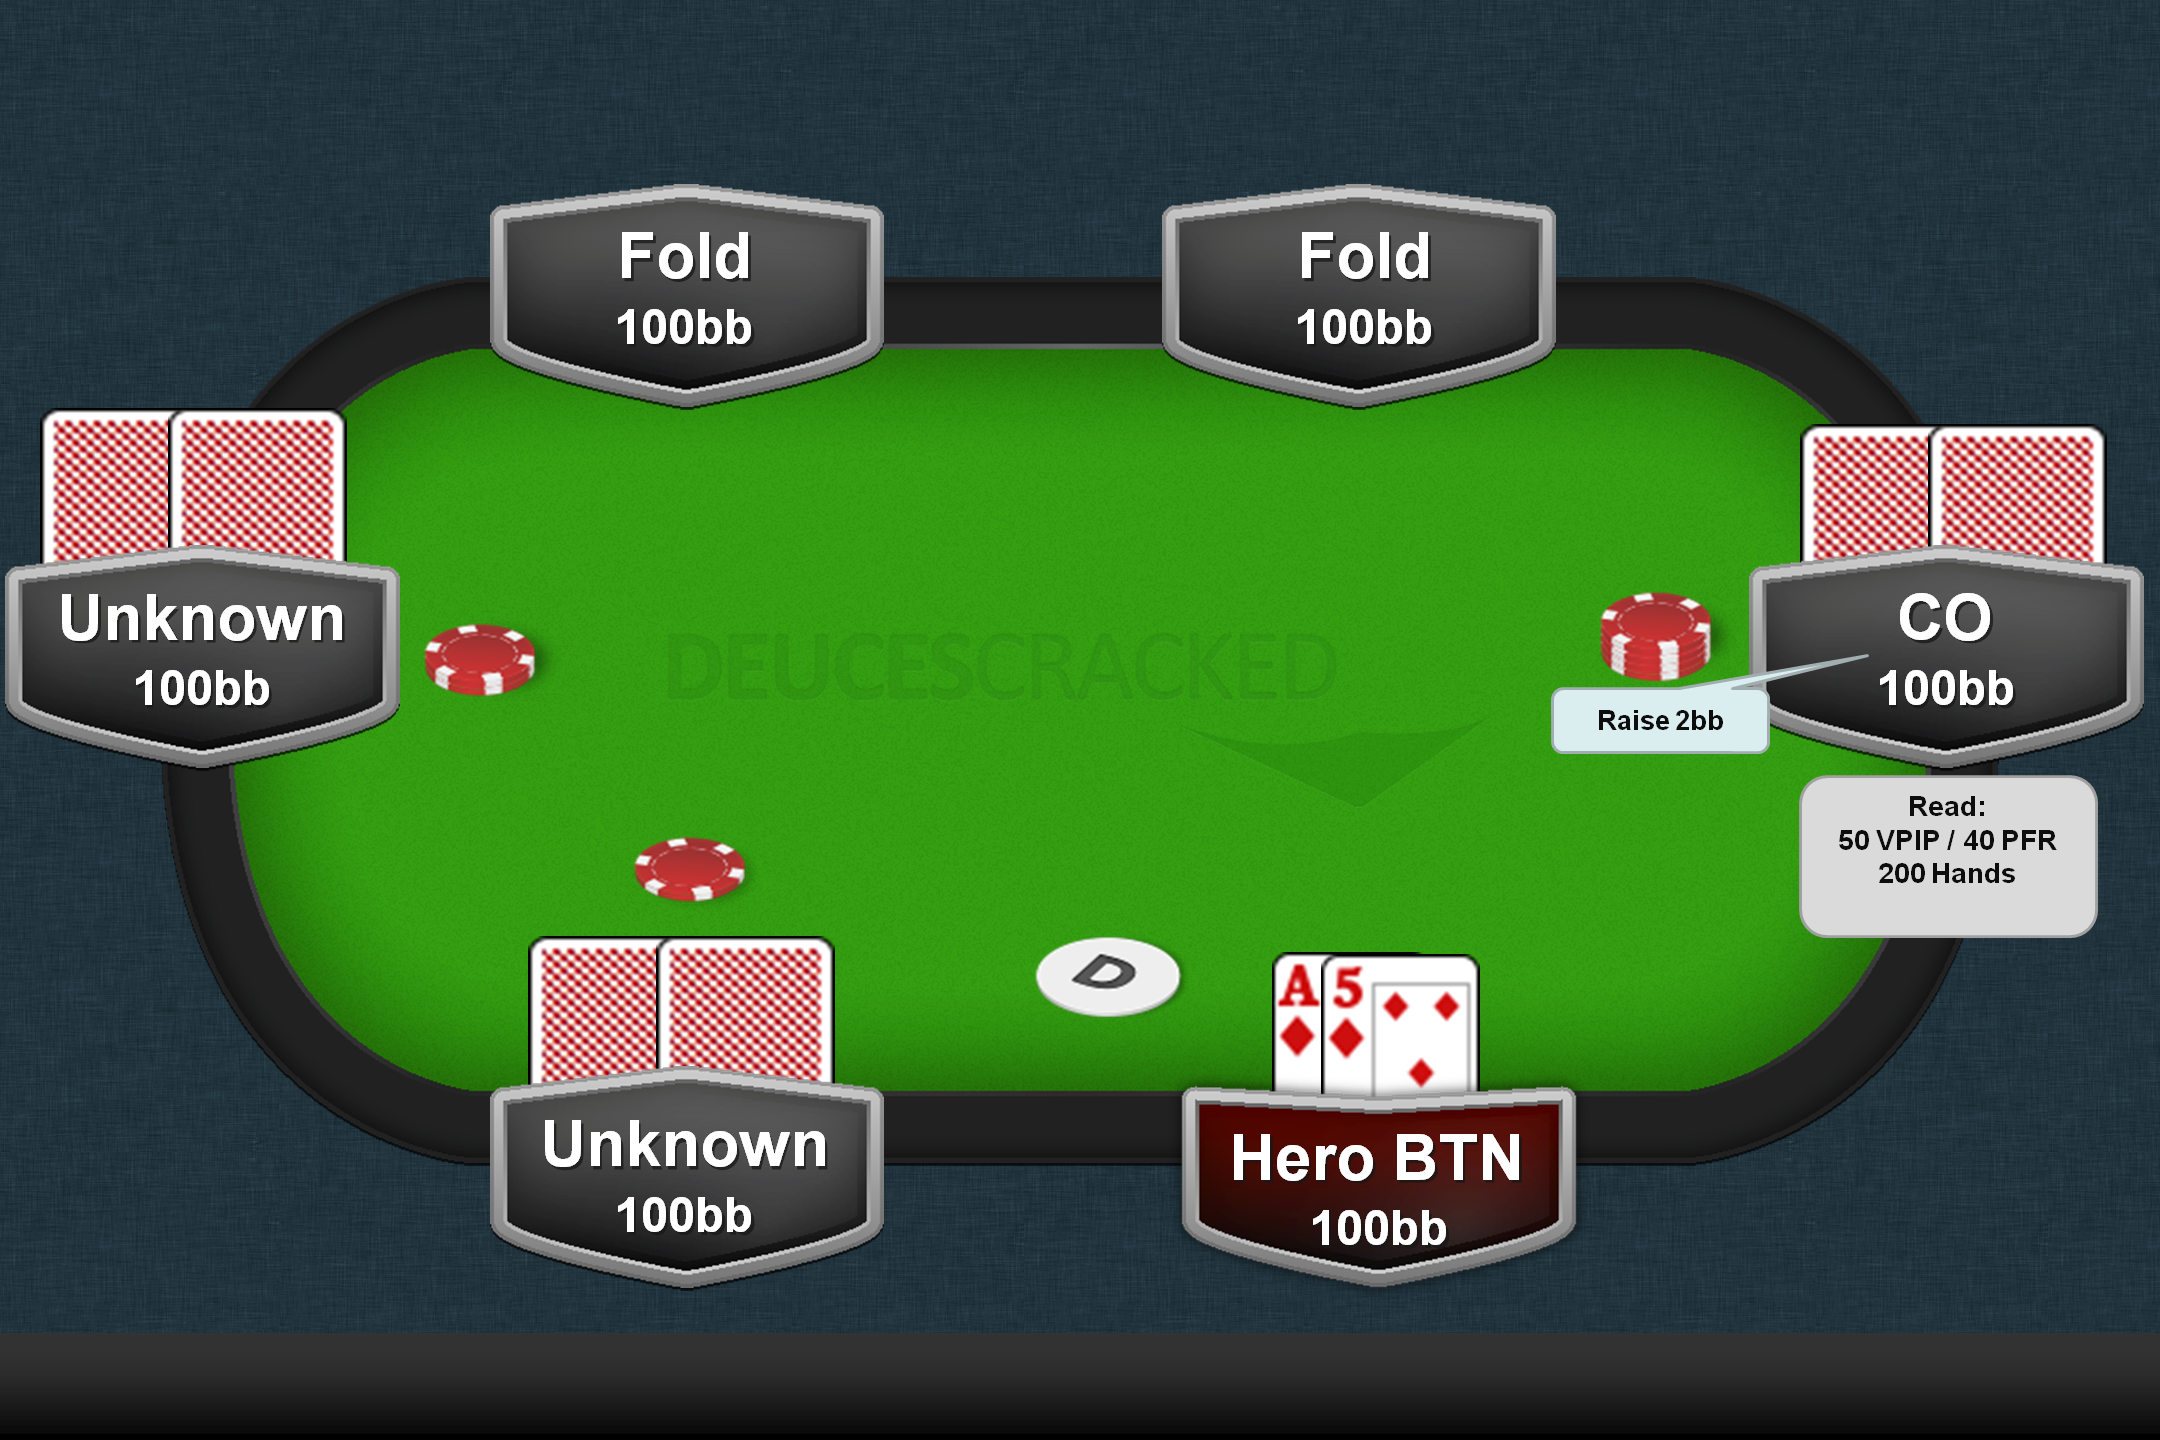
\includegraphics[keepaspectratio=true,width=.75\paperwidth]{Isolate.png}
\end{frame}


\section{Fold Equity}
\begin{frame}
\frametitle{Fold Equity}
\begin{itemize}
\item Gives 2 ways of winning the pot \pause
\item People who open too loosely \pause
\item As a deterrent \pause
\item Fold equity is responsible for most of $E[3B]$ \pause
\item A note on future videos \pause
\item Some people fold too frequently to 3-bets \pause
\item $\frac{\text{risk}}{\text{risk}+\text{reward}}$
\end{itemize}
\end{frame}

\subsection{$\frac{\text{risk}}{\text{risk}+\text{reward}}$}
\begin{frame}
\frametitle{$\frac{\text{risk}}{\text{risk}+\text{reward}}$}
\begin{itemize}
\item CO opens to 3bb, folded to Hero (BB) who 3-bets to 9.5bb (pot)
\item Pot odds = \pause 8.5: \pause 4.5 \pause
\item Risking \pause 8.5 \pause
\item To Win (Reward) \pause 4.5 \pause
\item $\frac{\text{risk}}{\text{risk}+\text{reward}} = \pause \frac{8.5}{8.5+4.5} \pause \approx 0.65$ \pause
\item If villain folds $> 65\%$ hero can 3-bet and muck if villain doesn't fold, and still profit. \pause
\item $E[\text{3B/muck}] = \pause P(\text{villain folds})E[\text{villain folds}] + \pause \;\;\;\;\;\;\;\;\;\;\;\;\;\;\;\;\;\;\;\;\;\;\;P(\text{villain doesn't fold})E[\text{muck}]$ \pause
\item $E[\text{3B/muck}] =  \pause 0.65\cdot \cancel{E[4.5]}(4.5) +  \pause 0.35\cdot \cancel{E[-8.5]}(-8.5)$
\item $\approx 0$
\end{itemize}
\end{frame}



\section{Preying Off Weakness}
\begin{frame}
\frametitle{Preying Off Weakness}
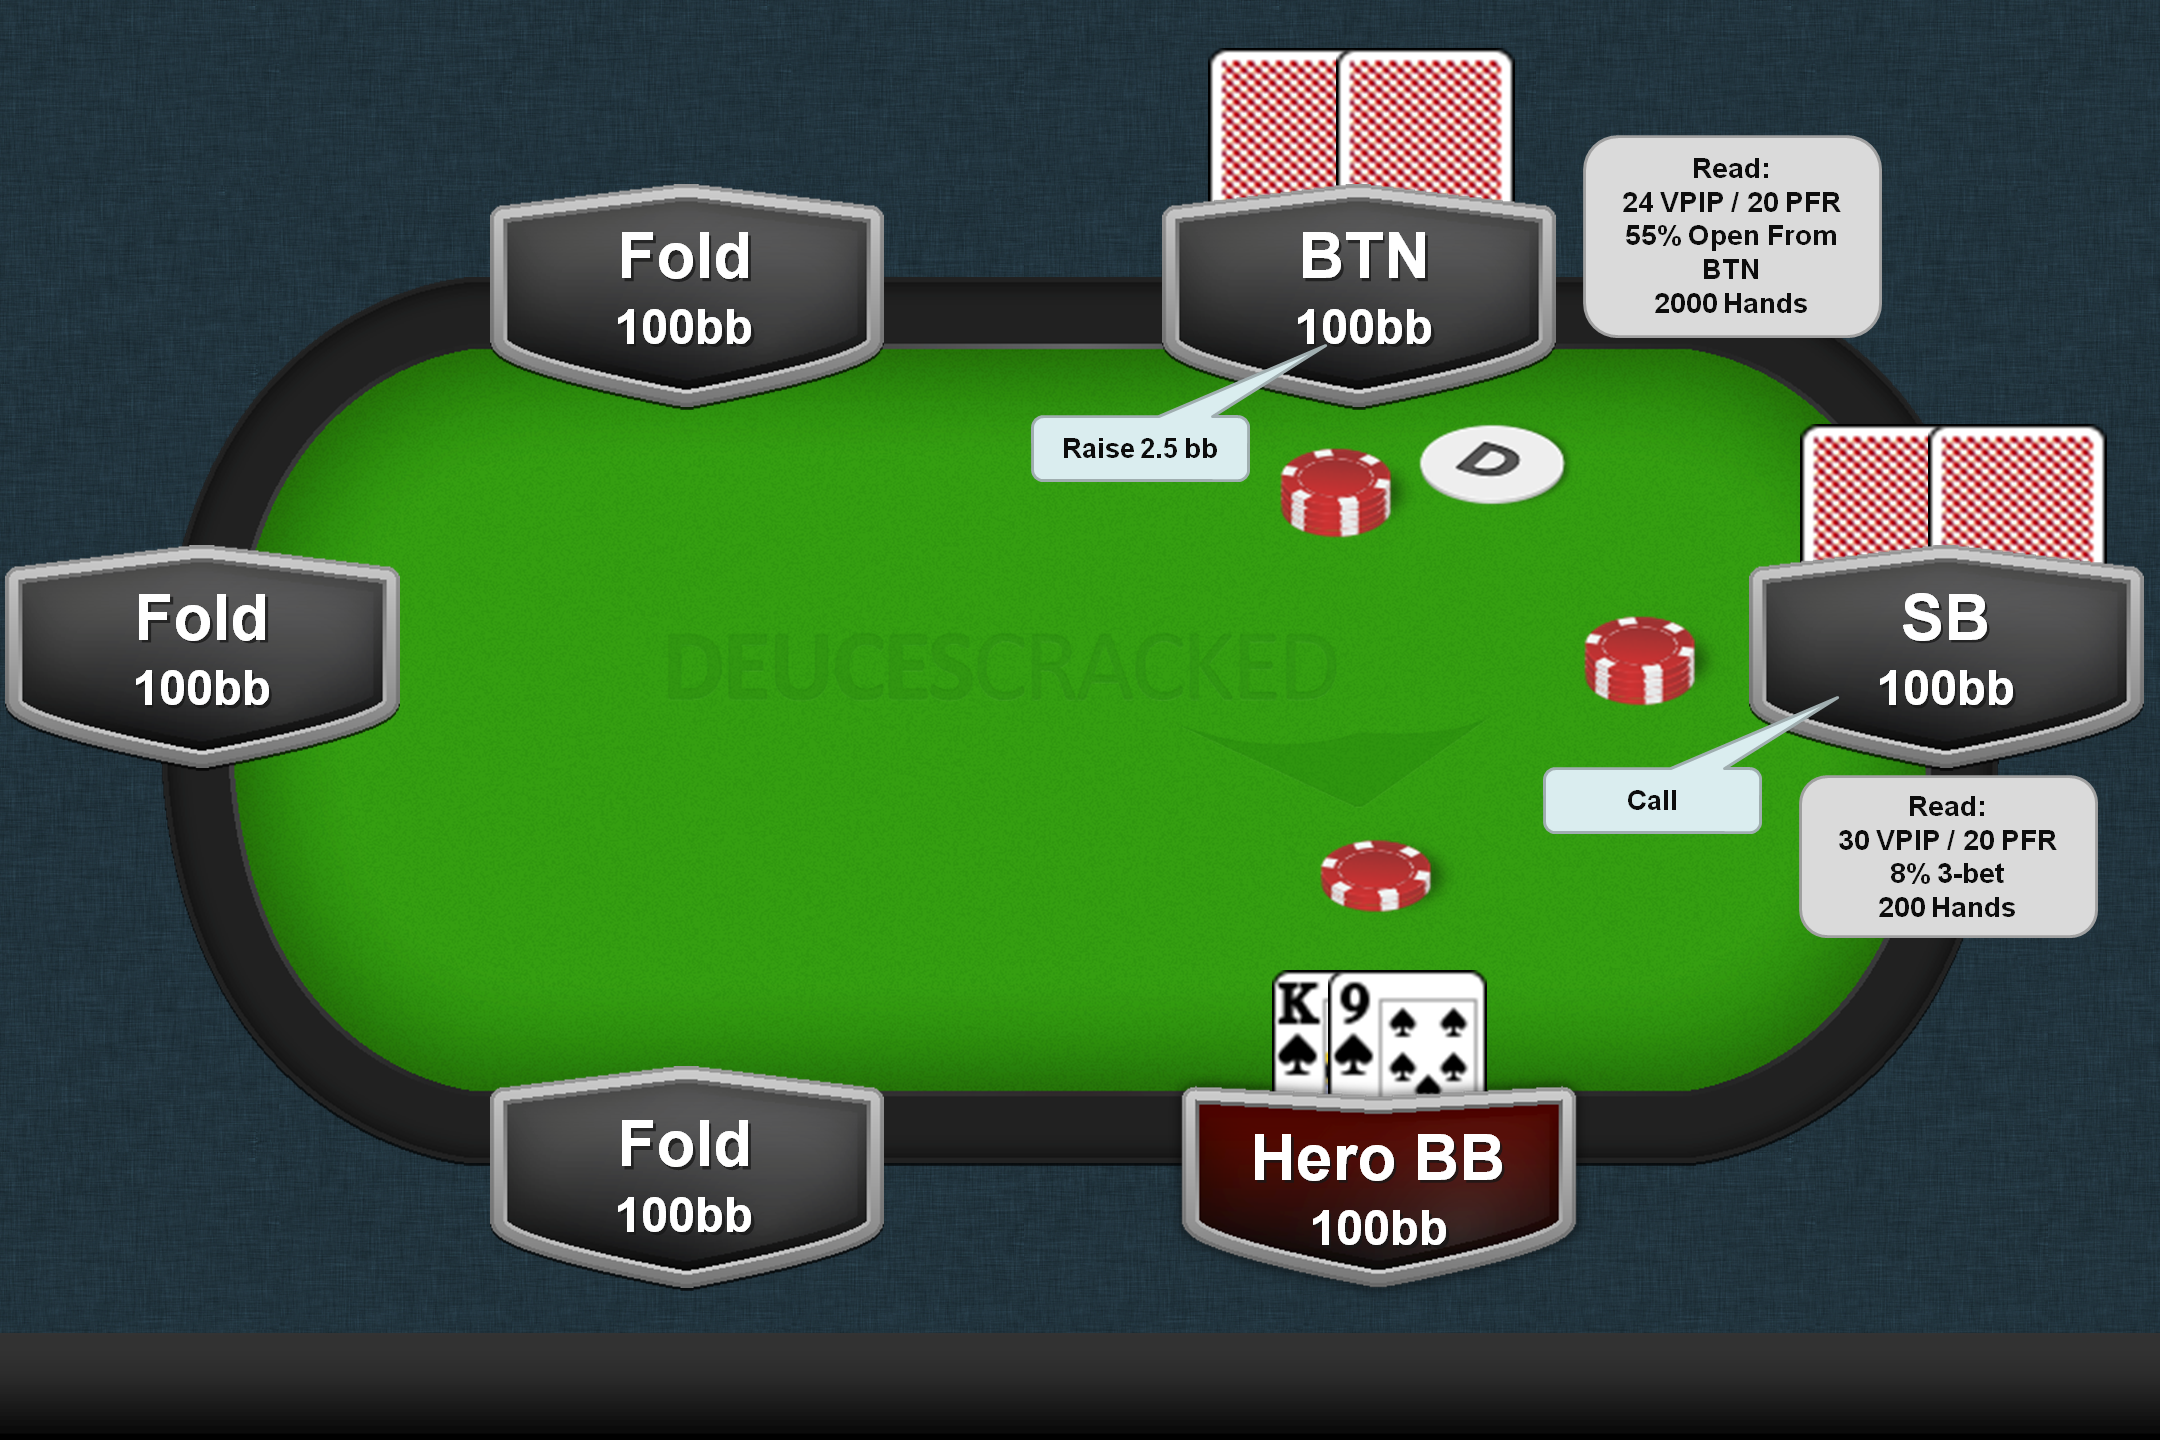
\includegraphics[keepaspectratio=true,width=.75\paperwidth]{Weakness.png}
\end{frame}

\section{Big Pots with Big Hands}
\begin{frame}
\frametitle{Big Pots with Big Hands}
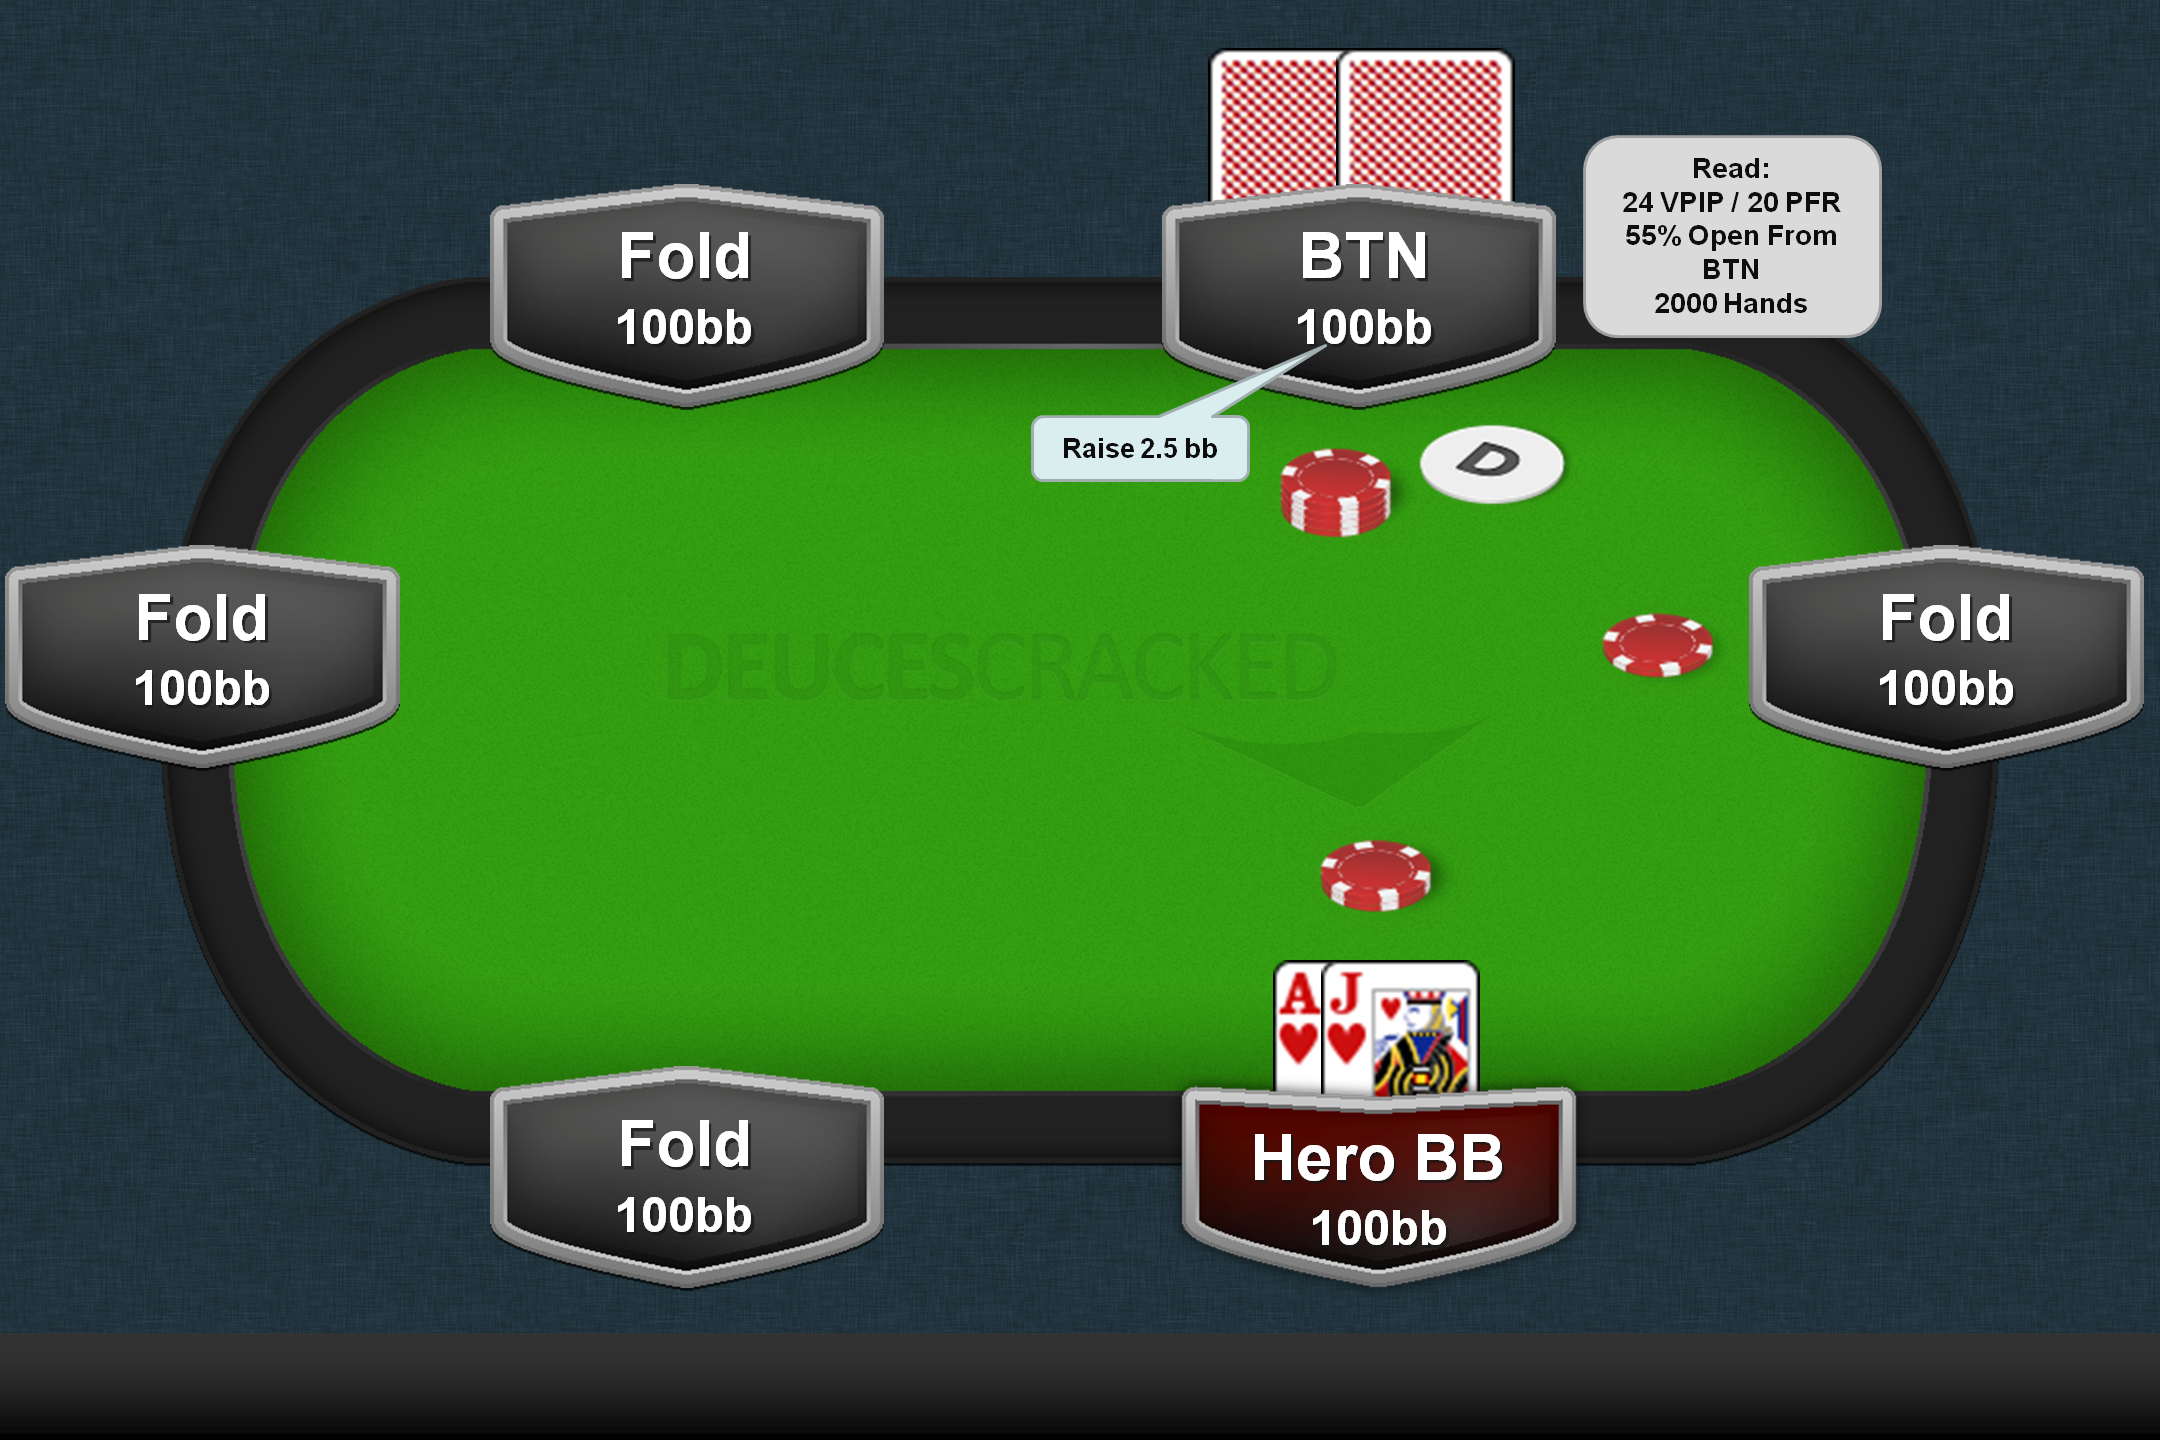
\includegraphics[keepaspectratio=true,width=.75\paperwidth]{Value.png}
\end{frame}

\section{Stack:Pot Ratio and Being OOP}
\begin{frame}
\frametitle{Stack:Pot Ratio and Being OOP}

\begin{itemize}
\item Assume: we bet the same \% of pot on flop, turn, and river \pause
\item (why it's not a terrible assumption) \pause
\item The \% that gets us all-in on the river: \pause
\item BTN Raises 2.5x, SB Folds, Hero(BB)...

\tikzset{blocknode/.style={inner sep=0,text width=0.5\textwidth,below right}}

\begin{block}{\tikz{\node[blocknode] {Action};\node[blocknode] at (0.24\textwidth,0){Pot}; \node[blocknode] at (0.4\textwidth,0){Stack}; \node[blocknode] at (0.6\textwidth,0){SPR};\node[blocknode] at (0.75\textwidth,0){\% Pot Bets};}}
\begin{tikzpicture}
\node[blocknode] {
Call \\
\noindent 3-Bet
};
\node[blocknode] at (0.24\textwidth,0) {
$\;\;6.0$ \\
\noindent $16.5$
};
\node[blocknode] at (0.4\textwidth,0) {
$97.5$ \\
\noindent $92.0$
};
\node[blocknode] at (0.6\textwidth,0) {
$16.3$ \\
\noindent $\;\;5.6$
};
\node[blocknode] at (0.75\textwidth,0) {
$111\%$ \\
\noindent $\;\;65\%$
};
\end{tikzpicture}
\end{block}

\vspace{5mm}
\pause
\item BTN Raises 2.5x, SB Calls, Hero(BB)...

\begin{block}{\tikz{\node[blocknode] {Action};\node[blocknode] at (0.24\textwidth,0){Pot}; \node[blocknode] at (0.4\textwidth,0){Stack}; \node[blocknode] at (0.6\textwidth,0){SPR};\node[blocknode] at (0.75\textwidth,0){\% Pot Bets};}}
\begin{tikzpicture}
\node[blocknode] {
Call \\
\noindent 3-Bet
};
\node[blocknode] at (0.24\textwidth,0) {
$\;\;7.5$ \\
\noindent $22.5$
};
\node[blocknode] at (0.4\textwidth,0) {
$97.5$ \\
\noindent $90.0$
};
\node[blocknode] at (0.6\textwidth,0) {
$13.0$ \\
\noindent $\;\;4.0$
};
\node[blocknode] at (0.75\textwidth,0) {
$100\%$ \\
\noindent $\;\;54\%$
};
\end{tikzpicture}
\end{block}
\end{itemize}


\end{frame}

\section{EV is Magnified}
\begin{frame}
\frametitle{EV is Magnified}
\begin{itemize}
\item Raising the stakes (infinite stacks) \pause
\item Finite stacks
\end{itemize}
\end{frame}

\end{document}

